\chapter{Introduction}
\label{chap:introduction}

The proliferation of commodity cloud services poses new opportunities and
challenges for hosting data.  On the one hand, the availability of
professionally-maintained infrastructure is a boon to developers, since it
offloads a large operational burden for maintaining application data.  On the other
hand, it is difficult to make effective use of this infrastructure over long
timescales.  Services can appear and disappear, services change their APIs and
storage semantics unilaterally, and the trust relationships between users and
services can change on a user-by-user basis.

This thesis presents a novel storage architecture for wide-area applications
that leverage commodity cloud services.  In our architecture,
developers specify their \emph{storage semantics} independently of
both the application and the infrastructure.  The storage semantics define the
rules for processing the application's reads and writes.  They are portable
across multiple services, and defined in a way that makes them easy to deploy
on a user-by-user basis and reuse in new contexts.

We present our design principles (Chapter~\ref{chap:design-principles}),
two production implementations (Chapter~\ref{chap:syndicate-sds}), sample
applications built under this architecture (Chapter~\ref{chap:applications}),
and early performance numbers that measure the overhead of our systems versus
leveraging cloud services directly (Chapter~\ref{chap:evaluation}).

\section{The Systems-of-Systems Approach}

Wide-area applications are \emph{systems-of-systems}.  
Systems-of-system applications are built by aggregating
functionality across multiple unrelated network applications into a coherent whole.
The most prominent example is the Internet, whereby multiple autonomous networks
are linked together by peering agreements to transport packets from any
connected host to any other connected host.  Another example is university
campus Webmail, which combines DNS, SMTP servers, Webmail application servers, and 
and a university-wide identity and authentication system to grant students and
faculty access to their email in their Web browsers
(Figure~\ref{fig:chap1-system-of-systems}).

\begin{figure}[h]
   \caption{Webmail is a system-of-systems wide-area application.  In order for
   Alice to receive an email from Bob, her university's DNS and SMTP servers
   must coordinate with the global DNS and SMTP networks, and her university's
   identity service and Webmail servers must coordinate to deliver her mail to
   her Web browser.}
   \centering
   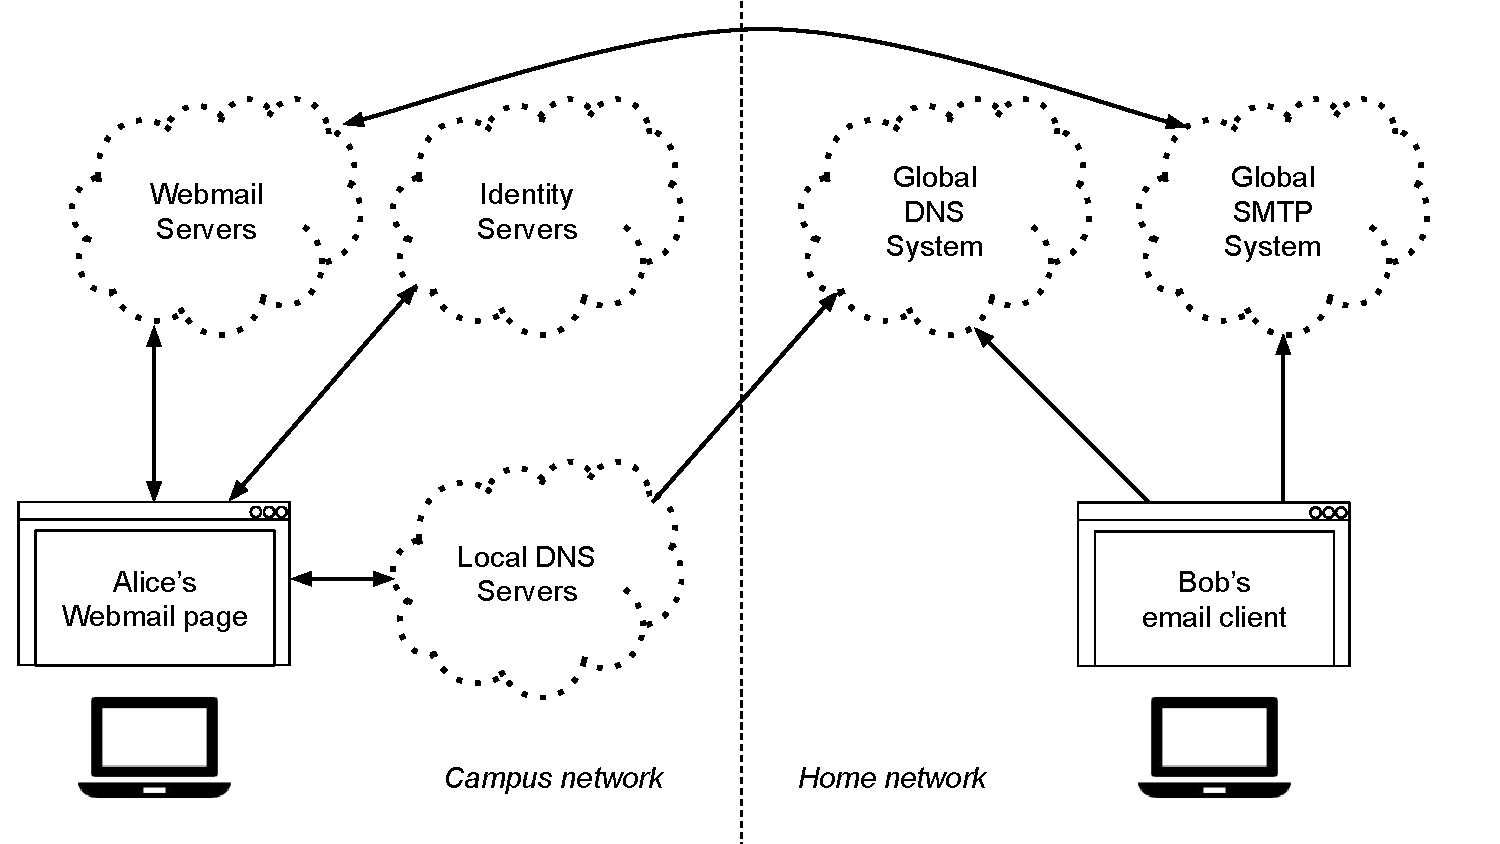
\includegraphics[width=0.9\textwidth,page=1]{figures/dissertation-figures}
   \label{fig:chap1-system-of-systems}
\end{figure}

Systems-of-systems application developers stand to benefit
from leveraging existing systems instead of building new, bespoke ones from
scratch.  An application can make use of one or more \textbf{cloud storage}
providers to host its data, and can distribute it to a scalable number of readers via one or more \textbf{content
distribution networks} (CDNs).  In addition, it can leverage data from
one or more external \textbf{curated data-sets} to provide better value to users.
For example, a navigation application like OpenStreetMap~\cite{openstreetmap} would host its users'
preferred routes, maps, and historic queries to the storage providers of their choice,
use a CDN to pre-fetch and cache map data to its appropriate geographic regions,
and use public weather data aggregated by NOAA~\cite{noaa} to predict how long a commute may take.

One significant side-effect of building systems-of-systems applications
is that a non-trivial amount of implementation effort goes towards
preserving end-to-end storage semantics.  For example, Web
application servers must coordinate with downstream CDN nodes to ensure that
clients read fresh data.  As another example, scientific compute clusters at
different labs must establish trust in a shared single-sign-on service (like
InCommon~\cite{incommon}) to allow scientists in one lab to access data in
another lab.

Despite this extra effort, the benefits offerred by the system-of-systems
approach to application design are obvious.  By relying on existing infrastructure,
developers can reduce development time and focus primarily on their application's business
logic.  In addition, developers can amortize the operational cost of
maintaining infrastructure across a multitude of applications by using these
shared resources.  This translates to reducing the time it takes to build a
working system, leading to faster iteration on the application's development.

\subsection{Challenges}

This thesis addresses three long-term risks with the system-of-systems approach.
First, \emph{the underlying services are unreliable}.  They can unilaterally
change their pricing, feature-set, APIs, and availability.
Applications that rely on these services can break without warning,
and cost developers unforeseeable amounts of time and money.

This exact relationship between service clients and the service operators is often encoded
in the operator's terms of service.  Existing terms for popular services
explicitly state that the operators have the ability to affect unilateral
changes~\cite{amazon-tos}~\cite{google-tos}~\cite{dropbox-tos}.  For example,
Dropbox unilaterally broke its API from version 1 to version
2~\cite{dropbox-v2-api-psa}, and Twitter dropped its API only after non-trivial
applications were built to leverage it~\cite{twitter-api-deprecation-psa}.

The second problem is that \emph{the services are heterogeneous}.  Services that fill similar roles
do not offer compatible interfaces or semantics.
Without careful planning, the application can become tightly-coupled to the
services it uses by implicitly depending on it to behave a certain way.  For
example, a service designed to use a single Amazon S3 bucket may implicitly
depend on its sequential consistency, and may not be able to simply switch to
using Dropbox (which provides eventual
consistency)~\cite{consistency-comparison-cloud-storage}.
This creates unexpectedly high service switching costs, making it
difficult for developers to address service unreliability or move to better
offerrings.

The third problem is that \emph{systems-of-systems applications span multiple
organizational boundaries}.  Each organization is a set of computers that
adhere to a single data-hosting policy, which encompasses concerns such as
access controls to the data, the data's availability, the data's durability, and
so on.  Examples include the set of file servers in a university lab,
the set of personal devices owned by a user, and the set of workstations owned by a
corporation.

The difficulty of building an application that spans multiple organizations
is that each organization places its own degree of trust in the underlying
services and the other organizations that use them.  Application developers
need to respect each organizations' policies to ensure correct execution.
For example, systems like email allow each organization to enforce email
storage policies on its email servers.  As another example, federated social
media like Mastadon~\cite{mastadon} and federated chat protocols like
XMPP~\cite{xmpp} allow each server to set its own rules on which peers can
connect, and what kinds of data each server will host and relay.

\section{Wide-area Software-defined Storage}

Our solution is to port both applications and services to a shared
intermediate layer, fulfilling the role of an ``operating system kernel'' for
wide-area applications.
Instead of focusing on porting each application to each service, we focus on porting applications and
services to an intermediate layer.  We will have this intermediate layer mediate all
data interactions between applications and services.  The goal is that when a new service
is ported to this layer, all existing applications can make use of it without
modification.

We address inter-organizational coordination by introducing an
\emph{open-membership} subsystem used for registering user identities and authentication
credentials.  This subsystem, called a \emph{self-sovereign
identity service} (SSI service), is used to bootstrap trust between users and their
organizations.   We use the SSI service to design the layer to give each user the ability to
programmatically control how other users and hosts may access the data they
produce.

We call a system that implements this intermediate storage layer a
\textit{wide-area software-defined storage} system.  We will henceforth refer to
this concept as SDS (see Chapter~\ref{chap:related} for a disambiguation of the
term).  SDS operates across organizational boundaries while preserving each of
their data hosting policies, and
encapsulates the complexity of interacting with individual services.

SDS offers two key benefits over the stats quo.  First, it efficiently preserves
application-specific storage semantics in the face of changing storage APIs.
Applications can safely and unilaterally change their storage semantics without
requiring any modification to other applications or services, and
storage providers can safely and unilaterally change their APIs without
affecting applications or other services. 
Second, SDS removes the need for service operators and
application developers to coordinate to accomodate each other's hosting
policies.  Users ``own'' their data in SDS---the user that creates a data record
has unilateral control over which other users and hosts may access it, and has
unilateral control over its storage semantics.

We have built two SDS prototypes to validate the effectiveness of our approach,
as well as several sample applications.  One of our prototype
systems, called Syndicate, gives scientific application end-points a coherent read/write
filesystem view of their data and offers developers a UNIX-y programming model
for describing the storage semantics their applications need.  Our other
prototype system, called Gaia, gives Web aplication endpoints a key/value store
that allows each user to host their own portion of the application state.

\section{Contributions}

In formulating, designing, and evaluating our SDS systems and sample applications,
we make the following contributions.

\begin{itemize}

\item We present the design principles of software-defined storage, framed in
terms of prior work and the real-world storage needs of existing applications.
We show how to minimize the man-hours required to keep applications compatible
with existing services while both preserving end-to-end storage semantics and
respecting each organization's data-hosting policies (Chatper~\ref{chap:design_principles}).

\item We present the design and implementation of two SDS systems: Gaia and
Syndicate.  Syndicate is a real SDS system being deployed in scientific
workflows today, and Gaia is a real SDS system being deployed to build
``serverless'' Web applications (i.e. Web applications that can operate
without the need for application-specific servers).
We show how Gaia and Syndicate make use of SDS design principles
(Chapter~\ref{chap:syndicate_sds}).

\item We show how to build SDS-powered applications.  We present the design and
implementation of non-trivial SDS-powered applications \emph{that could not
have been feasibly built without SDS}.  Among these are an end-to-end encrypted
Webmail client that removes the user from key management, a server-less
groupware application that lets users control how their data gets hosted and
accessed, and a scientific data-staging application that
automatically makes fresh datasets available from existing data repositories to
HPC clusters via commodity CDNs.  In all cases, we reuse each
service-specific patch across all applications
(Chapter~\ref{chap:applications}).

\item We present early performance numbers for Gaia and Syndicate, both in the
form of microbenchmarks and in real-world performance of applications built on
top of them (Chapter~\ref{chap:evaluation}).

\end{itemize}

